\documentclass{article}
\usepackage{fullpage,amssymb,amsmath,epsf,amsthm}
\usepackage[12pt]{extsizes}
\usepackage{psfrag}
\usepackage{graphicx}
\usepackage{enumerate}
\usepackage{hyperref}

\newcommand{\loss}{\mathsf{L}}
\newcommand{\represent}{\phi}
\newcommand{\mc}[1]{\mathcal{#1}}
\newcommand{\half}{\frac{1}{2}}

\newcommand{\newsec}{\section}
\newcommand{\denselist}{\itemsep 0pt\partopsep 0pt}
\newcommand{\bitem}{\begin{itemize}\denselist}
\newcommand{\eitem}{\end{itemize}}
\newcommand{\benum}{\begin{enumerate}\denselist}
\newcommand{\eenum}{\end{enumerate}}

\newcommand{\fig}[1]{\private{\begin{center}
{\Large\bf ({#1})}
\end{center}}}

\newcommand{\cpsf}[1]{{\centerline{\psfig{#1}}}}
\newcommand{\mytitle}[1]{\centerline{\LARGE\bf #1}}

\newcommand{\myw}{{\bf w}}

\newcommand{\mypar}[1]{\vspace{1ex}\noindent{\bf {#1}}}

\def\thmcolon{\hspace{-.85em} {\bf :} }

\newtheorem{THEOREM}{Theorem}[section]
\newenvironment{theorem}{\begin{THEOREM} \thmcolon }%
                        {\end{THEOREM}}
\newtheorem{LEMMA}[THEOREM]{Lemma}
\newenvironment{lemma}{\begin{LEMMA} \thmcolon }%
                      {\end{LEMMA}}
\newtheorem{COROLLARY}[THEOREM]{Corollary}
\newenvironment{corollary}{\begin{COROLLARY} \thmcolon }%
                          {\end{COROLLARY}}
\newtheorem{PROPOSITION}[THEOREM]{Proposition}
\newenvironment{proposition}{\begin{PROPOSITION} \thmcolon }%
                            {\end{PROPOSITION}}
\newtheorem{DEFINITION}[THEOREM]{Definition}
\newenvironment{definition}{\begin{DEFINITION} \thmcolon \rm}%
                            {\end{DEFINITION}}
\newtheorem{CLAIM}[THEOREM]{Claim}
\newenvironment{claim}{\begin{CLAIM} \thmcolon \rm}%
                            {\end{CLAIM}}
\newtheorem{EXAMPLE}[THEOREM]{Example}
\newenvironment{example}{\begin{EXAMPLE} \thmcolon \rm}%
                            {\end{EXAMPLE}}
\newtheorem{REMARK}[THEOREM]{Remark}
\newenvironment{remark}{\begin{REMARK} \thmcolon \rm}%
                            {\end{REMARK}}
%\newenvironment{proof}{\noindent {\bf Proof:} \hspace{.677em}}%
%                      {}

%theorem
\newcommand{\thm}{\begin{theorem}}
%lemma
\newcommand{\lem}{\begin{lemma}}
%proposition
\newcommand{\pro}{\begin{proposition}}
%definition
\newcommand{\dfn}{\begin{definition}}
%remark
\newcommand{\rem}{\begin{remark}}
%example
\newcommand{\xam}{\begin{example}}
%corollary
\newcommand{\cor}{\begin{corollary}}
%proof
\newcommand{\prf}{\noindent{\bf Proof:} }
%end theorem
\newcommand{\ethm}{\end{theorem}}
%end lemma
\newcommand{\elem}{\end{lemma}}
%end proposition
\newcommand{\epro}{\end{proposition}}
%end definition
\newcommand{\edfn}{\bbox\end{definition}}
%end remark
\newcommand{\erem}{\bbox\end{remark}}
%end example
\newcommand{\exam}{\bbox\end{example}}
%end corollary
\newcommand{\ecor}{\end{corollary}}
%end proof
\newcommand{\eprf}{\bbox\vspace{0.1in}}
%begin equation
\newcommand{\beqn}{\begin{equation}}
%end equation
\newcommand{\eeqn}{\end{equation}}

%\newcommand{\eqref}[1]{Eq.~\ref{#1}}

\newcommand{\KB}{\mbox{\it KB\/}}
\newcommand{\infers}{\vdash}
\newcommand{\sat}{\models}
\newcommand{\bbox}{\vrule height7pt width4pt depth1pt}

\newcommand{\act}[1]{\stackrel{{#1}}{\rightarrow}}
\newcommand{\at}[1]{^{(#1)}}

\newcommand{\argmax}{{\rm argmax}}

\newcommand{\rimp}{\Rightarrow}
\newcommand{\dimp}{\Leftrightarrow}

\newcommand{\bX}{\mbox{\boldmath $X$}}
\newcommand{\bY}{\mbox{\boldmath $Y$}}
\newcommand{\bZ}{\mbox{\boldmath $Z$}}
\newcommand{\bU}{\mbox{\boldmath $U$}}
\newcommand{\bE}{\mbox{\boldmath $E$}}
\newcommand{\bx}{\mbox{\boldmath $x$}}
\newcommand{\be}{\mbox{\boldmath $e$}}
\newcommand{\by}{\mbox{\boldmath $y$}}
\newcommand{\bz}{\mbox{\boldmath $z$}}
\newcommand{\bu}{\mbox{\boldmath $u$}}
\newcommand{\bd}{\mbox{\boldmath $d$}}
\newcommand{\smbx}{\mbox{\boldmath $\scriptstyle x$}}
\newcommand{\smbd}{\mbox{\boldmath $\scriptstyle d$}}
\newcommand{\smby}{\mbox{\boldmath $\scriptstyle y$}}
\newcommand{\smbe}{\mbox{\boldmath $\scriptstyle e$}}


\newcommand{\word}[1]{\mbox{\it #1\/}}
\newcommand{\Action}{\word{Action}}
\newcommand{\Proposition}{\word{Proposition}}
\newcommand{\true}{\word{true}}
\newcommand{\false}{\word{false}}
\newcommand{\Pre}{\word{Pre}}
\newcommand{\Add}{\word{Add}}
\newcommand{\Del}{\word{Del}}
\newcommand{\Result}{\word{Result}}
\newcommand{\Regress}{\word{Regress}}
\newcommand{\Maintain}{\word{Maintain}}

\newcommand{\bor}{\bigvee}
\newcommand{\invert}[1]{{#1}^{-1}}

\newcommand{\commentout}[1]{}

\newcommand{\bmu}{\mbox{\boldmath $\mu$}}
\newcommand{\btheta}{\mbox{\boldmath $\theta$}}
\newcommand{\IR}{\mbox{$I\!\!R$}}

\newcommand{\tval}[1]{{#1}^{1}}
\newcommand{\fval}[1]{{#1}^{0}}

\newcommand{\tr}{{\rm tr}}
\newcommand{\vecy}{{\vec{y}}}
\renewcommand{\Re}{{\mathbb R}}

\def\twofigbox#1#2{%
\noindent\begin{minipage}{\textwidth}%
\epsfxsize=0.35\maxfigwidth
\noindent \epsffile{#1}\hfill
\epsfxsize=0.35\maxfigwidth
\epsffile{#2}\\
\makebox[0.35\textwidth]{(a)}\hfill\makebox[0.35\textwidth]{(b)}%
\end{minipage}}

\def\twofigboxcd#1#2{%
\noindent\begin{minipage}{\textwidth}%
\epsfxsize=0.35\maxfigwidth
\noindent \epsffile{#1}\hfill
\epsfxsize=0.35\maxfigwidth
\epsffile{#2}\\
\makebox[0.35\textwidth]{(c)}\hfill\makebox[0.35\textwidth]{(d)}%
\end{minipage}}

\def\twofigboxnolabel#1#2{%
\begin{minipage}{\textwidth}%
\epsfxsize=0.35\maxfigwidth
\noindent \epsffile{#1}\hfill
\epsfxsize=0.35\maxfigwidth
\epsffile{#2}\\
%\makebox[0.48\textwidth]{(a)}\hfill\makebox[0.48\textwidth]{(b)}%
\end{minipage}
}

\def\twofigboxnolabelFive#1#2{%
\begin{minipage}{\textwidth}%
\hbox to 0.5in{}\epsfxsize=0.35\maxfigwidth
\noindent \epsffile{#1}\hfill
\epsfxsize=0.35\maxfigwidth
\epsffile{#2}\hbox to 0.5in{}\\
%\makebox[0.48\textwidth]{(a)}\hfill\makebox[0.48\textwidth]{(b)}%
\end{minipage}
}

\def\threefigbox#1#2#3{%
\noindent\begin{minipage}{\textwidth}%
\epsfxsize=0.33\maxfigwidth
\noindent \epsffile{#1}\hfill
\epsfxsize=0.33\maxfigwidth
\noindent \epsffile{#2}\hfill 
\epsfxsize=0.33\maxfigwidth
\epsffile{#3}\\
\makebox[0.31\textwidth]{{\scriptsize (a)}}\hfill%
\makebox[0.31\textwidth]{{\scriptsize (b)}}\hfill
\makebox[0.31\textwidth]{{\scriptsize (c)}}%
\smallskip
\end{minipage}}

\def\threefigboxnolabel#1#2#3{%
\noindent\begin{minipage}{\textwidth}%
\epsfxsize=0.33\maxfigwidth
\noindent \epsffile{#1}\hfill
\epsfxsize=0.33\maxfigwidth
\noindent \epsffile{#2}\hfill 
\epsfxsize=0.33\maxfigwidth
\epsffile{#3}\\
%\makebox[0.31\textwidth]{{\scriptsize (a)}}\hfill%
%\makebox[0.31\textwidth]{{\scriptsize (b)}}\hfill
%\makebox[0.31\textwidth]{{\scriptsize (c)}}%
%\smallskip
\end{minipage}}

\newlength{\maxfigwidth}
\setlength{\maxfigwidth}{\textwidth}
%\def\captionsize {\footnotesize}
\def\captionsize {}

\newcommand{\xsi}{{x^{(i)}}}
\newcommand{\xsd}{{x^{(d)}}}
\newcommand{\xsj}{{x^{(j)}}}
\newcommand{\ysi}{{y^{(i)}}}
\newcommand{\ysj}{{y^{(j)}}}
\newcommand{\gsi}{{\gamma^{(i)}}}
\newcommand{\wsi}{{w^{(i)}}}
\newcommand{\esi}{{\epsilon^{(i)}}}

\newcommand{\calM}{{\cal M}}
\newcommand{\calH}{{\cal H}}
\newcommand{\calN}{{\cal N}}
\newcommand{\calX}{{\cal X}}
\newcommand{\calY}{{\cal Y}}
\newcommand{\calL}{{\cal L}}
\newcommand{\calP}{{\cal P}}
\newcommand{\calD}{{\cal D}}
\newcommand{\calF}{{\cal F}}

\newcommand{\ytil}{{\tilde{y}}}

\newcommand{\Ber}{{\rm Bernoulli}}
\newcommand{\MI}{{\rm MI}}
\newcommand{\E}{{\rm E}}

\newcommand{\pstar}{{p^{\ast}}}
\newcommand{\bstar}{{b^{\ast}}}
\newcommand{\dstar}{{d^{\ast}}}
\newcommand{\wstar}{{w^{\ast}}}
\newcommand{\alphastar}{\alpha^{\ast}}
\newcommand{\alphastari}{{\alpha_i^{\ast}}}
\newcommand{\betastar}{{\beta^{\ast}}}
\newcommand{\tol}{{\textit tol}}
\newcommand{\phihat}{\hat\phi}
\newcommand{\ehat}{\hat\varepsilon}
\newcommand{\hhat}{\hat{h}}
\newcommand{\hstar}{h^\ast}
\newcommand{\VC}{{\rm VC}}

\newcommand{\Strain}{S_{\rm train}}
\newcommand{\Scv}{{S_{\rm cv}}}

\newcommand{\hwb}{{h_{w,b}}}


\begin{document}
\title{XCS229i Supplemental Lecture Notes}
\author{Andrew Ng}
%\date{Lectures from 1/7/03 to 1/16/03}
\date{}
\maketitle

\section{General loss functions}

Building off of our interpretations of supervised learning as (1) choosing a
representation for our problem, (2) choosing a loss function, and (3)
minimizing the loss, let us consider a slightly more general formulation for
supervised learning.  In the supervised learning settings we have considered
thus far, we have input data $x \in \R^n$ and targets $y$ from a space
$\mc{Y}$. In linear regression, this corresponded to $y \in \R$, that is,
$\mc{Y} = \R$, for logistic regression and other binary classification
problems, we had $y \in \mc{Y} = \{-1, 1\}$, and for multiclass
classification we had $y \in \mc{Y} = \{1, 2, \ldots, k\}$ for some number
$k$ of classes.

For each of these problems, we made predictions based on $\theta^T x$ for
some vector $\theta$, and we constructed a loss function $\loss : \R \times
\mc{Y} \to \R$, where $\loss(\theta^T x, y)$ measures the loss we suffer for
predicting $\theta^T x$. For logistic regression, we use the logistic loss
\begin{equation*}
  \loss(z, y) = \log(1 + e^{-y z})
  ~~ \mbox{or} ~~
  \loss(\theta^T x, y) = \log(1 + e^{-y \theta^T x}).
\end{equation*}
For linear regression we use the squared error
\begin{equation*}
  \loss(z, y) = \half (z - y)^2
  ~~ \mbox{or} ~~
  \loss(\theta^T x, y) = \half (\theta^T x - y)^2.
\end{equation*}
For multiclass classification, we had a slight variant, where we let
$\Theta = [\theta_1 ~ \cdots ~ \theta_k]$ for $\theta_i \in \R^n$, and
used the loss $\loss : \R^k \times \{1, \ldots, k\} \to \R$
\begin{equation*}
  \loss(z, y) = \log\left(\sum_{i = 1}^k \exp(z_i - z_y)\right)
  ~~ \mbox{or} ~~
  \loss(\Theta^T x, y) = \log\left(\sum_{i = 1}^k 
  \exp(x^T(\theta_i - \theta_y))\right),
\end{equation*}
the idea being that we wish to have $\theta_y^T x > \theta_i^T x$ for
all $i \neq k$.
Given a training set of pairs $\{x^{(i)}, y^{(i)}\}$, choose $\theta$
by minimizing the empirical risk
\begin{equation}
  \label{eqn:empirical-risk}
  J(\theta) = \frac{1}{m} \sum_{i = 1}^m \loss(\theta^T \xsi, \ysi).
\end{equation}

\section{The representer theorem}

\renewenvironment{proof}{\noindent{\bf Proof}\hspace*{1em}}{\qed\bigskip\\}

\newcommand{\reg}{r}
\newcommand{\norm}[1]{\left\|{#1}\right\|}
\newcommand{\normbigg}[1]{\bigg\|{#1}\bigg\|}
\newcommand{\ltwo}[1]{\norm{#1}_2}
\newcommand{\ltwobigg}[1]{\normbigg{#1}_2}

Let us consider a slight variant of choosing $\theta$ to minimize the
risk~\eqref{eqn:empirical-risk}. In many situations---for reasons that we
will study more later in the class---it is useful to add
\emph{regularization} to the risk $J$. We add regularization for many
reasons: often, it makes problem~\eqref{eqn:empirical-risk} easier to solve
numerically, and also it can allow the $\theta$ we get out of minimizing the
risk~\eqref{eqn:empirical-risk} able to generalize better to unseen data.
Generally, regularization is taken to be of the form
$\reg(\theta) = \norm{\theta}$ or $\reg(\theta) = \norm{\theta}^2$ for
some norm $\norm{\cdot}$ on $\R^n$.
The most common choice is so-called $\ell_2$-regularization, in which
we choose
\begin{equation*}
  \reg(\theta) = \frac{\lambda}{2} \ltwo{\theta}^2,
\end{equation*}
where we recall that $\ltwo{\theta} = \sqrt{\theta^T \theta}$ is the Euclidean
norm, or length, of the vector $\theta$.
This gives rise to the \emph{regularized risk}, which is
\begin{equation}
  \label{eqn:regularized-risk}
  J_\lambda(\theta) = \frac{1}{m} \sum_{i=1}^m \loss(\theta^T \xsi, \ysi)
  + \frac{\lambda}{2} \ltwo{\theta}^2.
\end{equation}

Let us consider the structure of any $\theta$ that minimizes the
risk~\eqref{eqn:regularized-risk}. We assume---as we often do---that for
each fixed target value $y \in \mc{Y}$, the function $\loss(z, y)$ is convex
in $z$. (This is the case for linear regression and binary and multiclass
logistic regression, as well as a number of other losses we will consider.)
It turns out that under these assumptions, we may always write the solutions
to the problem~\eqref{eqn:regularized-risk} as a \emph{linear combination}
of the input variables $\xsi$. More precisely, we have the following
theorem, known as the \emph{representer theorem}.
\begin{theorem}
  \label{theorem:representer}
  Suppose in the definition of the regularized
  risk~\eqref{eqn:regularized-risk} that $\lambda \ge 0$.  Then there is a
  minimizer of the regularized risk~\eqref{eqn:regularized-risk} that can be
  written
  \begin{equation*}
    \theta = \sum_{i = 1}^m \alpha_i \xsi
  \end{equation*}
  for some real-valued weights $\alpha_i$.
\end{theorem}
\begin{proof}
  For intuition, we give a proof of the result in the case that $\loss(z,
  y)$, when viewed as a function of $z$, is differentiable and $\lambda >
  0$.  In Appendix~\ref{appendix:representer}, we present a more general
  statement of the theorem as well as a rigorous proof.

  Let $\loss'(z, y) = \frac{\partial}{\partial z} \loss(z, y)$ denote the 
  derivative of the loss with respect to $z$. Then by the chain rule,
  we have the gradient identity
  \begin{equation*}
    \nabla_\theta \loss(\theta^T x, y)
    = \loss'(\theta^T x, y) x
    ~~ \mbox{and} ~~
    \nabla_\theta \half \ltwo{\theta}^2 = \theta,
  \end{equation*}
  where $\nabla_\theta$ denotes taking a gradient with respect to
  $\theta$. As the risk must have $0$ gradient at all stationary points
  (including the minimizer), we can write
  \begin{equation*}
    \nabla J_\lambda(\theta)
    = \frac{1}{m} \sum_{i = 1}^m \loss'(\theta^T \xsi, \ysi) \xsi
    + \lambda \theta = \vec{0}.
  \end{equation*}
  In particular, letting $w_i = \loss'(\theta^T \xsi, \ysi)$, as
  $\loss'(\theta^T \xsi, \ysi)$ is a scalar (which depends on $\theta$, but
  no matter what $\theta$ is, $w_i$ is still a real number),
  we have
  \begin{equation*}
    \theta = -\frac{1}{\lambda} \sum_{i = 1}^n w_i \xsi.
  \end{equation*}
  Set $\alpha_i = -\frac{w_i}{\lambda}$ to get the result.
\end{proof}

\section{Nonlinear features and kernels}

Based on the representer theorem, Theorem~\ref{theorem:representer},
we see that we can always write the vector $\theta$ as
a linear combination of the data $\{\xsi\}_{i=1}^m$. Importantly,
this means we can \emph{always} make predictions
\begin{equation*}
  \theta^T x = x^T \theta = \sum_{i = 1}^m \alpha_i x^T \xsi.
\end{equation*}
That is, in \emph{any} learning algorithm, we may can replace all
appearances of $\theta^T x$ with $\sum_{i = 1}^m \alpha_i \xsi^T x$,
and then minimize directly over $\alpha \in \R^m$.

Let us consider this idea in somewhat more generality. In our discussion of
linear regression, we had a problem in which the input $x$ was the living
area of a house, and we considered performing regression using the features
$x$, $x^2$ and $x^3$ (say) to obtain a cubic function.  To distinguish
between these two sets of variables, we'll call the ``original'' input value
the input {\bf attributes} of a problem (in this case, $x$, the living
area).  When that is mapped to some new set of quantities that are then
passed to the learning algorithm, we'll call those new quantities the input
{\bf features}.  (Unfortunately, different authors use different terms to
describe these two things, but we'll try to use this terminology
consistently in these notes.)  We will also let $\phi$ denote the {\bf
  feature mapping}, which maps from the attributes to the features.  For
instance, in our example, we had
\begin{equation*}
  \phi(x) = \left[\begin{matrix} x \\ x^2 \\ x^3 \end{matrix}\right].
\end{equation*}

Rather than applying a learning algorithm using the original input
attributes $x$, we may instead want to learn using some features $\phi(x)$.
To do so, we simply need to go over our previous algorithm, and replace $x$
everywhere in it with $\phi(x)$.

Since the algorithm can be written entirely in terms of the inner products
$\langle x, z \rangle$, this means that we would replace all those inner
products with $\langle \phi(x), \phi(z) \rangle$.  Specificically, given a
feature mapping $\phi$, we define the corresponding {\bf kernel} to be
\begin{equation*}
  K(x,z) = \phi(x)^T \phi(z).
\end{equation*}
Then, everywhere we previously had $\langle x, z \rangle$ in our algorithm,
we could simply replace it with $K(x,z)$, and our algorithm would now be
learning using the features $\phi$. Let us write this out more carefully.
We saw by the representer theorem (Theorem~\ref{theorem:representer})
that we can write $\theta = \sum_{i = 1}^m \alpha_i \phi(\xsi)$ for
some weights $\alpha_i$. Then we can write the (regularized) risk
\begin{align*}
  J_\lambda(\theta)
  & = J_\lambda(\alpha) \\
  & = \frac{1}{m} \sum_{i = 1}^m \loss\bigg(\phi(\xsi)^T
  \sum_{j = 1}^m \alpha_j \phi(x^{(j)}), \ysi\bigg)
  + \frac{\lambda}{2}
  \ltwobigg{\sum_{i = 1}^m
    \alpha_i \phi(\xsi) }^2 \\
  & = \frac{1}{m} \sum_{i = 1}^m \loss\bigg(
  \sum_{j = 1}^m \alpha_j \phi(\xsi)^T \phi(x^{(j)}), \ysi\bigg)
  + \frac{\lambda}{2}
  \sum_{i = 1}^m
  \sum_{j = 1}^m
  \alpha_i \alpha_j \phi(\xsi)^T \phi(x^{(j)}) \\
  & = \frac{1}{m} \sum_{i = 1}^m \loss\bigg(
  \sum_{j = 1}^m \alpha_j K(\xsi, x^{(j)}), \ysi\bigg)
  + \frac{\lambda}{2} \sum_{i, j} \alpha_i \alpha_i K(\xsi, x^{(j)}).
\end{align*}
That is, we can write the entire loss function to be minimized
in terms of the kernel matrix
\begin{equation*}
  K = [K(\xsi, x^{(j)})]_{i, j = 1}^m \in \R^{m \times m}.
\end{equation*}

Now, given $\phi$, we could easily compute $K(x,z)$ by finding $\phi(x)$ and
$\phi(z)$ and taking their inner product.  But what's more interesting is
that often, $K(x,z)$ may be very inexpensive to calculate, even though
$\phi(x)$ itself may be very expensive to calculate (perhaps because it is
an extremely high dimensional vector).  In such settings, by using in our
algorithm an efficient way to calculate $K(x,z)$, we can learn in the high
dimensional feature space space given by $\phi$, but without ever having to
explicitly find or represent vectors $\phi(x)$.
As a few examples, some kernels (corresponding to infinite-dimensional
vectors $\phi$) include
\begin{equation*}
  K(x, z) = \exp\left(-\frac{1}{2 \tau^2} \ltwo{x - z}^2\right),
\end{equation*}
known as the Gaussian or Radial Basis Function (RBF) kernel and applicable
to data in any dimension, or the min-kernel (applicable when
$x \in \R$, defined by
\begin{equation*}
  K(x, z) = \min\{x, z\}.
\end{equation*}
See also the lecture notes on Support Vector Machines (SVMs) for
more on these kernel machines.

\section{Stochastic gradient descent for kernelized machine learning}
\newcommand{\Ksi}{{K^{(i)}}}

If we let $K \in \R^{m \times m}$ denote the kernel matrix, and for shorthand
define the vectors
\begin{equation*}
  \Ksi = \left[\begin{matrix} K(\xsi, x^{(1)}) \\ K(\xsi, x^{(2)}) \\
      \vdots \\ K(\xsi, x^{(m)})\end{matrix}\right],
\end{equation*}
so that $K = [K^{(1)} ~ K^{(2)} ~ \cdots ~ K^{(m)}]$, then we may write
the regularized risk in a consise form as
\begin{align*}
  J_\lambda(\alpha)
  & = \frac{1}{m} \sum_{i = 1}^m \loss(\Ksi^T \alpha, \ysi)
  + \frac{\lambda}{2} \alpha^T K \alpha.
\end{align*}
Now, let us consider taking a stochastic gradient of the above risk
$J_\lambda$. That is, we wish to construct a (simple to compute) random
vector whose expectation is $\nabla J_\lambda(\alpha)$, which does not have
too much variance. 
To do so, we first compute the gradient of $J_\lambda(\alpha)$ on its own.
We calculate the gradient of individual loss terms by noting that
\begin{equation*}
  \nabla_\alpha \loss(\Ksi^T \alpha, \ysi)
  = \loss'(\Ksi^T \alpha, \ysi) \Ksi,
\end{equation*}
while
\begin{equation*}
  \nabla_\alpha \left[\frac{\lambda}{2} \alpha^T K\alpha
    \right]
  = \lambda K\alpha = \lambda \sum_{i = 1}^m \Ksi \alpha_i.
\end{equation*}
Thus, we have
\begin{equation*}
  \nabla_\alpha J_\lambda(\alpha)
  = \frac{1}{m} \sum_{i=1}^m \loss'(\Ksi^T\alpha, \ysi) \Ksi
  + \lambda \sum_{i=1}^m \Ksi \alpha_i.
\end{equation*}
Thus, if we choose a random index $i \in \{1, \ldots, m\}$, we have that
\begin{equation*}
  \loss'(\Ksi^T \alpha, \ysi) \Ksi + m \lambda \Ksi \alpha_i
\end{equation*}
is a stochastic gradient for $J_\lambda(\alpha)$.
This gives us a stochastic gradient procedure for Kernel supervised
learning problems, shown in Figure~\ref{fig:sgd-for-kernel}.
\begin{figure}[ht!]
  \begin{center}
    \algbox{
      \textbf{Input:} A loss function $\loss$,
        kernel matrix $K = [K^{(1)} ~ \cdots ~ K^{(m)}]$,
        and labels $\{\ysi\}_{i = 1}^m$, and sequence
        of positive stepsizes $\eta_1, \eta_2, \eta_3, \ldots$ \\

        \textbf{Iterate} for $t = 1, 2, \ldots$
        \begin{enumerate}[(i)]
        \item Choose index $i \in \{1, \ldots, m\}$ uniformly at random
        \item Update
          \begin{equation*}
            \alpha := \alpha -
            \eta_t \left[\loss'(\Ksi^T \alpha, \ysi) \Ksi
              + m \lambda \Ksi \alpha_i \right].
          \end{equation*}
        \end{enumerate}
    }
    \caption{\label{fig:sgd-for-kernel} Stochastic gradient descent
      for kernel supervised learning problems.}
  \end{center}
\end{figure}
One minor remark is in order regarding Algorithm~\ref{fig:sgd-for-kernel}:
because we multiply the $\lambda \Ksi \alpha_i$ term by $m$ to keep
the gradient unbiased, it is important that $\lambda > 0$ not be 
too large, as the algorithm can be a bit unstable otherwise. In
addition, a common choice of stepsize is to use $\eta_t = 1 / \sqrt{t}$,
or a constant multiple thereof.

\section{Support vector machines}
\newcommand{\hinge}[1]{\left[{#1}\right]_+}
% \newcommand{\normal}{\mathsf{N}}
\renewcommand{\E}{\mathbb{E}}

Now we discuss (one approach) to Support Vector Machines (SVM)s, which
apply to binary classification problems with labels
$y \in \{-1, 1\}$, and a particular choice of loss function $\loss$.
In particular, for the support vector machine, we use the margin-based
loss function
\begin{equation}
  \label{eqn:svm-loss}
  \loss(z, y)
  = \hinge{1 - yz} =
  \max\{0, 1 - yz\}.
\end{equation}
So, in a sense, SVMs are nothing but a special case of the general
theoretical results we have described above. In particular,
we have the empirical regularized risk
\begin{equation*}
  J_\lambda(\alpha)
  = \frac{1}{m} \sum_{i = 1}^m \hinge{1 - \ysi \Ksi^T \alpha}
  + \frac{\lambda}{2} \alpha^T K \alpha,
\end{equation*}
where the matrix $K = [K^{(1)} ~ \cdots ~ K^{(m)}]$ is
defined by $K_{ij} = K(x^{(i)}, x^{(j)})$.

In the lecture notes, you can see another way of deriving the support
vector machine and a description of why we actually call
them support vector machines.

\section{An example}

\begin{figure}[ht]
  \begin{center}
    \begin{tabular}{cc}
      \hspace{-2cm}
      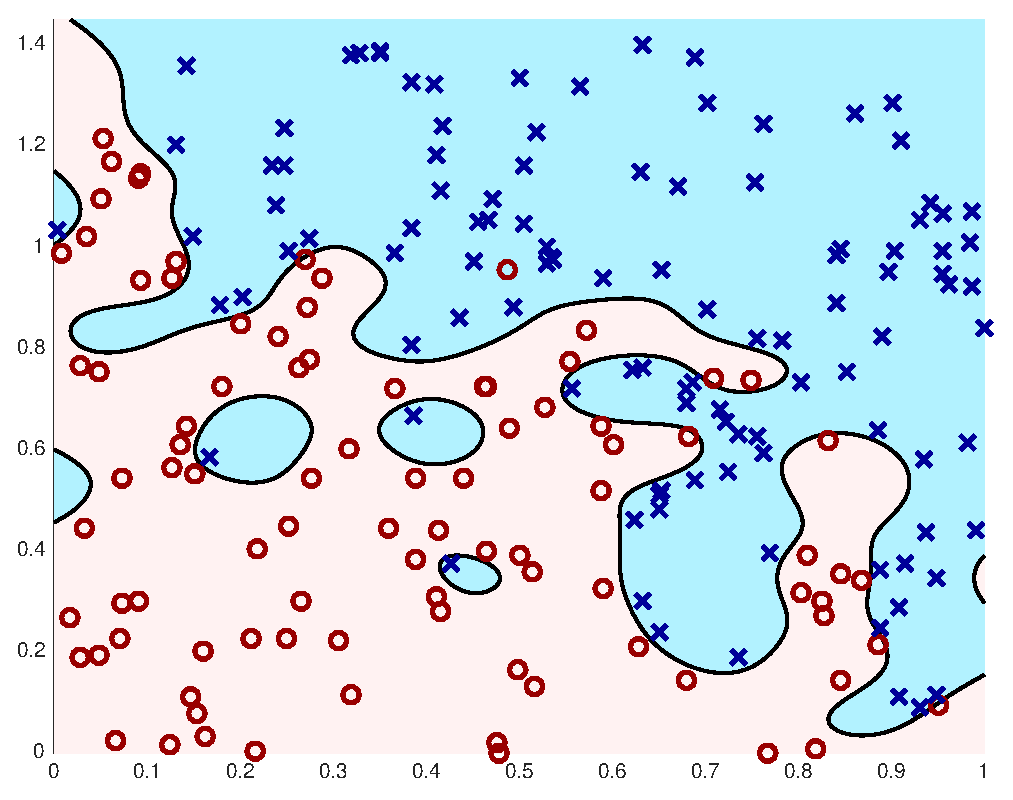
\includegraphics[width=.6\columnwidth,clip]{kernel_train_0.100.eps} &
      \hspace{-.5cm}
      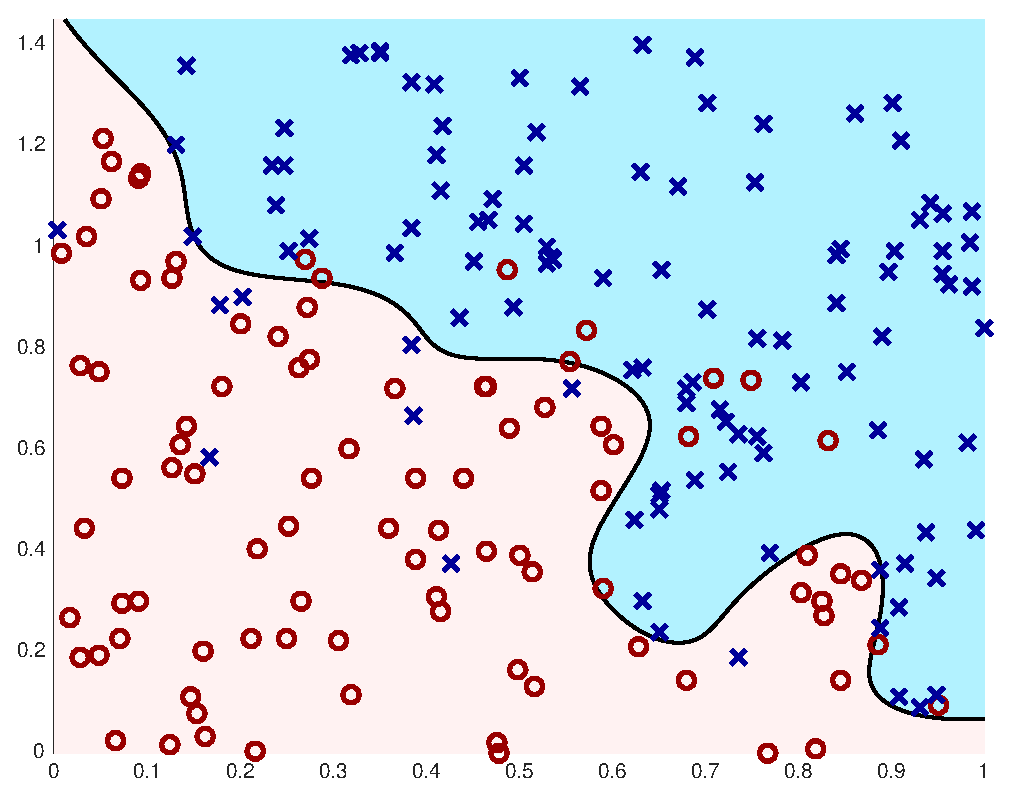
\includegraphics[width=.6\columnwidth,clip]{kernel_train_0.200.eps} \\
      \hspace{-2cm} $\tau = .1$ & \hspace{-.5cm} $\tau = .2$
    \end{tabular}
    \caption{\label{fig:kernel-bandwidths-small} Small bandwidths 
      $\tau$ for Gaussian kernel  $K(x, z) = \exp(-\frac{1}{2 \tau^2}
      \ltwo{x - z}^2)$.}
  \end{center}
\end{figure}

\begin{figure}[ht]
  \begin{center}
    \begin{tabular}{cc}
      \hspace{-2cm}
      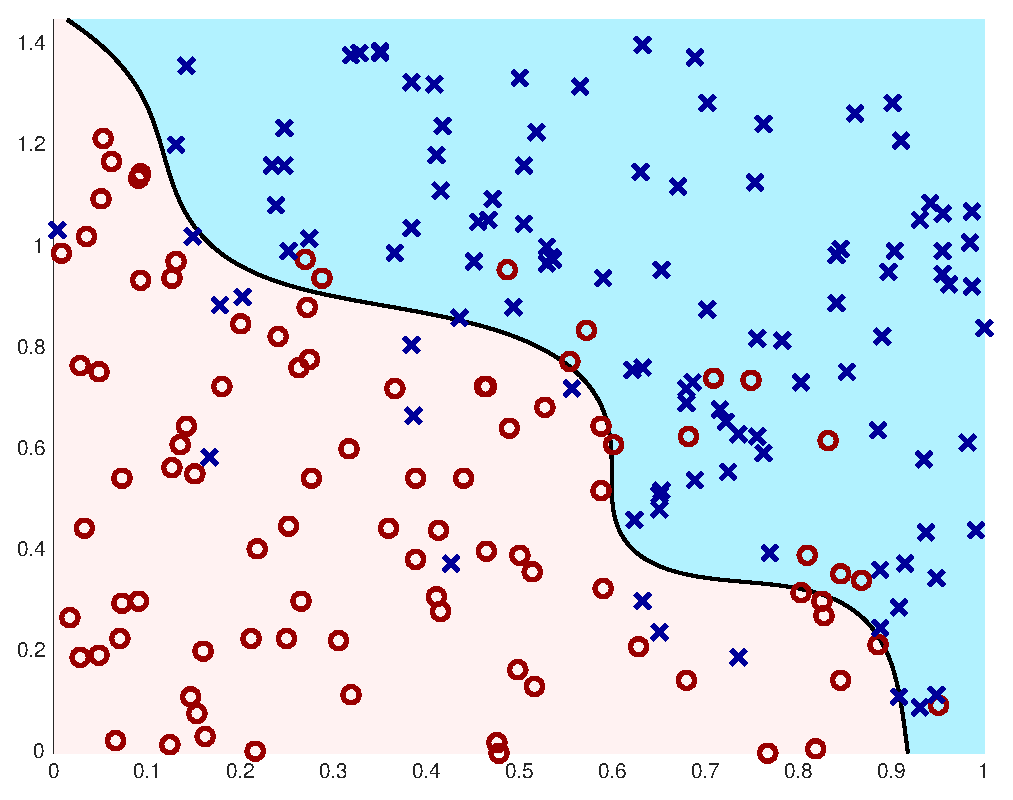
\includegraphics[width=.6\columnwidth,clip]{kernel_train_0.400.eps} &
      \hspace{-.5cm}
      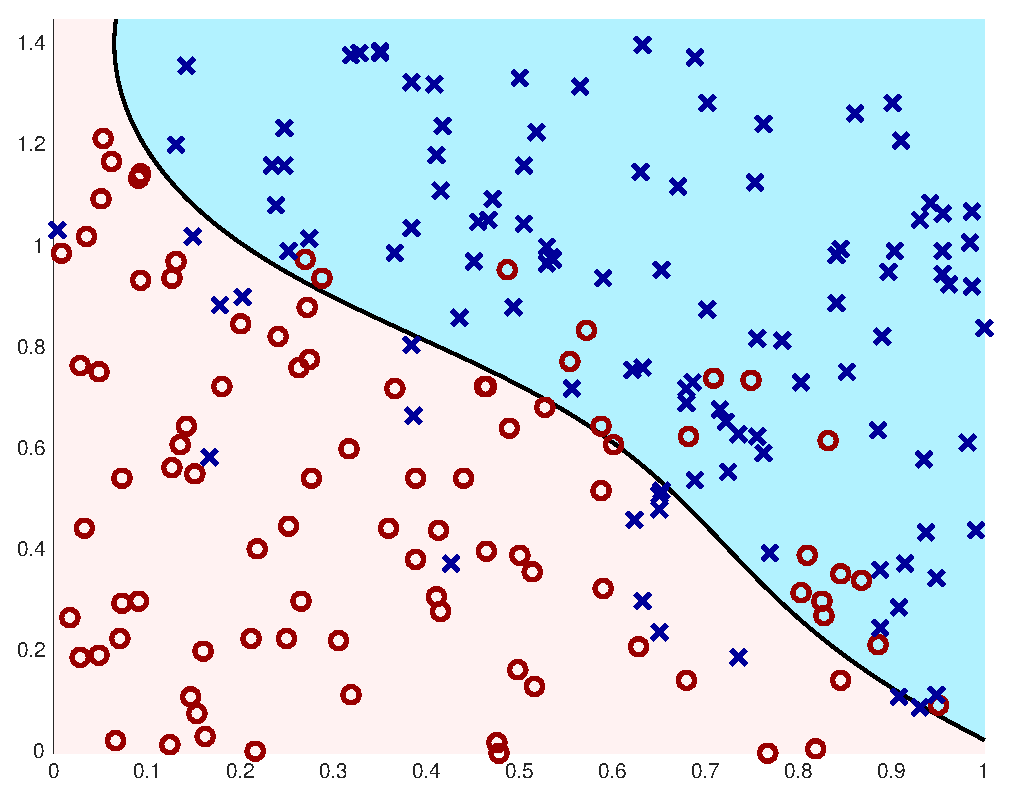
\includegraphics[width=.6\columnwidth,clip]{kernel_train_0.800.eps} \\
      \hspace{-2cm} $\tau = .4$ & \hspace{-.5cm} $\tau = .8$
    \end{tabular}
    \caption{\label{fig:kernel-bandwidths-medium} Medium bandwidths
      $\tau$ for Gaussian kernel $K(x, z) = \exp(-\frac{1}{2 \tau^2}
      \ltwo{x - z}^2)$.}
  \end{center}
\end{figure}
\begin{figure}[ht]
  \begin{center}
    \begin{tabular}{cc}
      \hspace{-2cm}
      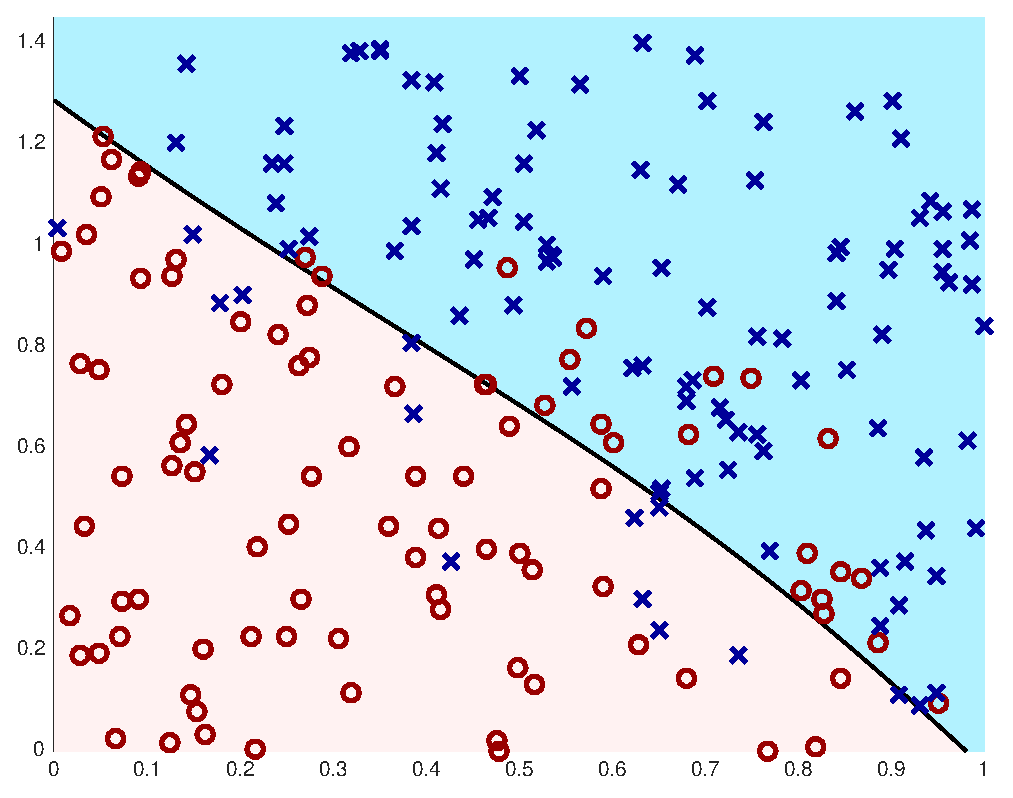
\includegraphics[width=.6\columnwidth,clip]{kernel_train_1.600.eps} &
      \hspace{-.5cm}
      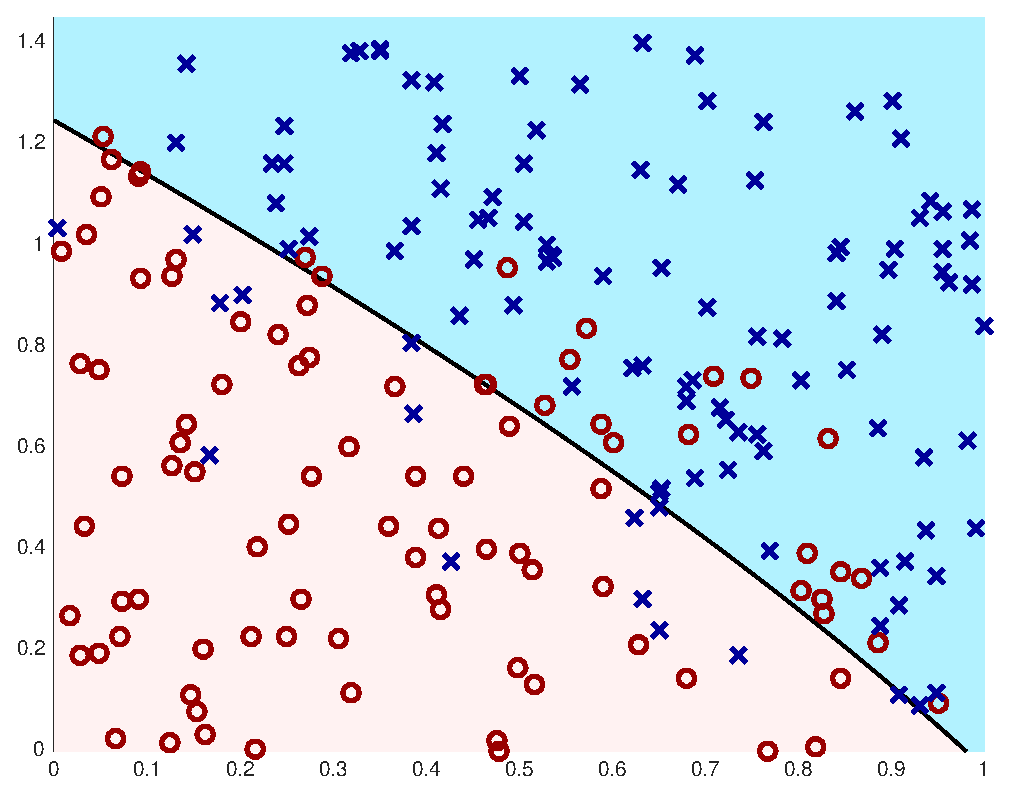
\includegraphics[width=.6\columnwidth,clip]{kernel_train_3.200.eps} \\
      \hspace{-2cm} $\tau = 1.6$ & \hspace{-.5cm} $\tau = 3.2$
    \end{tabular}
    \caption{\label{fig:kernel-bandwidths-large}
      Large bandwidths $\tau$ for Gaussian kernel
      $K(x, z) = \exp(-\frac{1}{2 \tau^2} \ltwo{x - z}^2)$.}
  \end{center}
\end{figure}

In this section, we consider a particular example kernel, known as the
Gaussian or Radial Basis Function (RBF) kernel. This kernel is defined by
\begin{equation}
  \label{eqn:rbf-kernel}
  K(x, z) = \exp\left(-\frac{1}{2 \tau^2} \ltwo{x - z}^2\right),
\end{equation}
where $\tau > 0$ is a parameter controlling the \emph{bandwidth} of the
kernel. Intuitively, for $\tau$ very small, we will have $K(x, z) \approx 0$
unless $x \approx z$, that is, $x$ and $z$ are very close, in which case we
have $K(x, z) \approx 1$. However, for $\tau$ large, then we have a much
smoother kernel function $K$.  The feature function $\represent$ for this
kernel is infinite dimensional.\footnote{If you have seen characteristic
  functions or Fourier transforms, then you might recognize the RBF kernel
  as the Fourier transform of the Gaussian distribution with mean zero and
  variance $\tau^2$. That is, in $\R^n$, let $W \sim \normal(0, \tau^2 I_{n
    \times n})$, so that $W$ has density $p(w) = \frac{1}{(2 \pi
    \tau^2)^{n/2}} \exp(-\frac{\ltwo{w}^2}{2 \tau^2})$.  Let $i = \sqrt{-1}$
  be the imaginary unit, then for any vector $v$ we have
  \begin{align*}
    \E[\exp(i v^T W)]
    = \int \exp(i v^T w) p(w) dw
    & = \int \frac{1}{(2 \pi \tau^2)^{n/2}}
    \exp\left(i v^T w - \frac{1}{2 \tau^2} \ltwo{w}^2\right) dw \\
    & = \exp\left(-\frac{1}{2 \tau^2} \ltwo{v}^2 \right).
  \end{align*}
  Thus, if we define the ``vector'' (really, function)
  $\phi(x, w) = e^{i x^T w}$ and let $a^*$ be the complex
  conjugate of $a \in \mathbb{C}$, then we have
  \begin{equation*}
    \E[\phi(x, W) \phi(z, W)^*]
    = \E[e^{i x^T W} e^{-i x^T W}]
    % = \int e^{i x^T w} e^{-i z^T w} p(w) dw
    = \E[\exp(i W^T (x - z))]
    = \exp\left(-\frac{1}{2 \tau^2} \ltwo{x - z}^2\right).
  \end{equation*}
  In particular, we see that $K(x, z)$ is the inner product
  in a space of functions that are integrable against $p(w)$.
}
That said, it is possible to gain some intuition for the kernel
by considering the classifications it makes on a new example $x$:
we have prediction
\begin{equation*}
  \sum_{i = 1}^m K(\xsi, x) \alpha_i
  = \sum_{i = 1}^m \exp\left(-\frac{1}{2 \tau^2} \ltwo{\xsi - x}^2\right)
  \alpha_i,
\end{equation*}
so that this becomes something like a weighting depending on
\emph{how close} $x$ is to each $\xsi$---that is, the contribution
of weight $\alpha_i$ is multiplied by the similarity of $x$ to $\xsi$
as determined by the kernel function.

\begin{figure}[ht]
  \begin{center}
    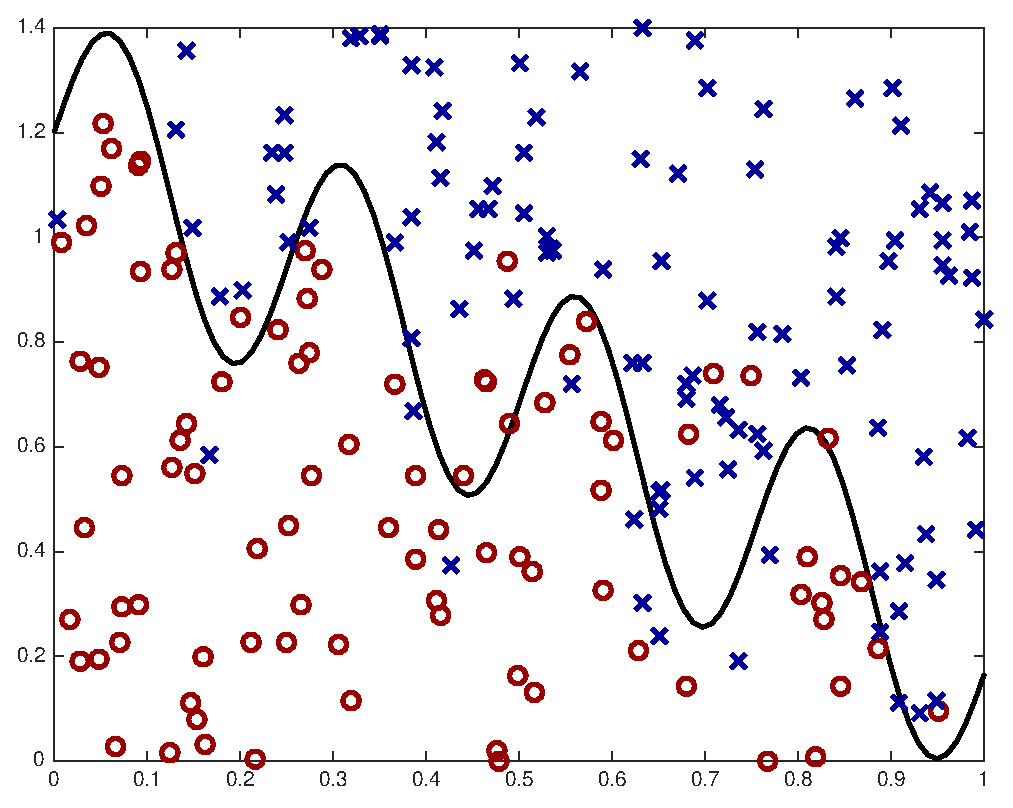
\includegraphics[width=.6\columnwidth]{true_class.eps}
    \caption{\label{fig:true-classifier} Optimal classifier along
      with training data.}
  \end{center}
\end{figure}

In Figures~\ref{fig:kernel-bandwidths-small}, \ref{fig:kernel-bandwidths-medium},
and~\ref{fig:kernel-bandwidths-large},
we show the results of training
$6$ different kernel classifiers by minimizing
\begin{equation*}
  J_\lambda(\alpha) = \sum_{i = 1}^m \hinge{1 - \ysi\Ksi^T \alpha}
  + \frac{\lambda}{2} \alpha^T K \alpha,
\end{equation*}
with $m = 200$ and $\lambda = 1/m$, for different values
of $\tau$ in the kernel~\eqref{eqn:rbf-kernel}. We plot the
training data (positive examples as blue \texttt{x}'s and
negative examples as red \texttt{o}'s) as well as the decision surface
of the resulting classifier. That is, we plot the lines defined by
\begin{equation*}
  \left\{x \in \R^2 ~ : ~ \sum_{i = 1}^m K(x, \xsi) \alpha_i = 0 \right\},
\end{equation*}
giving the regions where the learned classifier makes a prediction $\sum_{i
  = 1}^m K(x, \xsi) \alpha_i > 0$ and $\sum_{i = 1}^m K(x, \xsi) \alpha_i <
0$. From the figure, we see that for large $\tau$, we have a very simple
classifier: it is nearly linear, while for $\tau = .1$, the classifier has
substantial variability and is highly non-linear.
For reference, in Figure~\ref{fig:true-classifier}, we plot the
optimal classifier along with the training data; the optimal classifier
minimizes the misclassification error given infinite training data.

\appendix

\section{A more general representer theorem}

\label{appendix:representer}

In this section, we present a more general version of the representer
theorem along with a rigorous proof. Let $r : \R \to \R$ be any
non-decreasing function of its argument, and consider the regularized
risk
\begin{equation}
  \label{eqn:general-regularized-risk}
  J_r(\theta) = \frac{1}{m} \sum_{i=1}^m \loss(\xsi^T \theta, \ysi)
  + r(\ltwo{\theta}).
\end{equation}
Often, we take $r(t) = \frac{\lambda}{2} t^2$, which corresponds to the
common choice of $\ell_2$-regularization, but the next theorem
makes clear that this is not necessary for the representer theorem.
Indeed, we could simply take $r(t) = 0$ for all $t$, and the theorem
still holds.
\begin{theorem}[Representer theorem in $\R^n$]
  \label{theorem:real-representer}
  Let $\theta \in \R^n$ be any vector. Then there exists
  some $\alpha \in \R^m$ and
  $\theta^{(\alpha)} = \sum_{i = 1}^m \alpha_i \xsi$ such that
  \begin{equation*}
    J_r(\theta^{(\alpha)}) \le J_r(\theta).
  \end{equation*}
\end{theorem}
\noindent
In particular, there is no loss of generality in always assuming we can
write the optimization problem to minimize $J(\theta)$ by only considering
$\theta$ in the span of the data.

\begin{proof}
  Our proof relies on some machinery from linear algebra, which allows
  us to keep it concise, but feel free to ask questions if it is
  too concise.

  The vectors $\{\xsi\}_{i = 1}^m$ are in $\R^n$,
  and as a consequence there is some subspace $V$ of $\R^n$
  such that
  \begin{equation*}
    V = \bigg\{\sum_{i = 1}^m \beta_i \xsi : \beta_i \in \R\bigg\}.
  \end{equation*}
  Then $V$ has an orthonormal basis $\{v_1, \ldots, v_{n_0}\}$ for vectors
  $v_i \in \R^n$, where the size (dimension) of the basis is $n_0 \le
  n$. Thus we can write $V = \{\sum_{i = 1}^{n_0} b_i v_i : b_i \in \R\}$,
  where we recall that orthonormality means that the vectors $v_i$ satisfy
  $\ltwo{v_i} = 1$ and $v_i^T v_j = 0$ for $i \neq j$.
  There is also an orthogonal subspace $V^\perp = \{u \in \R^n
  : u^Tv = 0 ~ \mbox{for~all~} v \in V\}$, which has an orthonormal basis
  of size $n_\perp = n - n_0 \ge 0$, which we write as
  $\{u_1, \ldots, u_{n_\perp}\} \subset \R^n$. By construction
  they satisfy $u_i^T v_j = 0$ for all $i, j$.

  Because $\theta \in \R^n$, we know that we can write it uniquely
  as
  \begin{equation*}
    \theta = \sum_{i = 1}^{n_0} \nu_i v_i
    + \sum_{i = 1}^{n_\perp} \mu_i u_i,
    ~~ \mbox{where} ~~ \nu_i \in \R ~ \mbox{and} ~
    \mu_i \in \R,
  \end{equation*}
  and the values $\mu, \nu$ are unique.
  Now, we know that by definition of the space $V$ as the
  span of $\{\xsi\}_{i=1}^m$, there exists $\alpha \in \R^m$ such that
  \begin{equation*}
    \sum_{i = 1}^{n_0} \nu_i v_i
    = \sum_{i = 1}^m \alpha_i \xsi,
  \end{equation*}
  so that we have
  \begin{equation*}
    \theta = \sum_{i = 1}^m \alpha_i \xsi + \sum_{i = 1}^{n_\perp} \mu_i u_i.
  \end{equation*}
  Define $\theta^{(\alpha)} = \sum_{i=1}^m \alpha_i \xsi$.  Now, for any
  data point $x^{(j)}$, we have
  \begin{equation*}
    u_i^T {x^{(j)}} = 0
    ~~ \mbox{for~all}~ i = 1, \ldots, n_\perp,
  \end{equation*}
  so that $u_i^T \theta^{(\alpha)} = 0$.
  As a consquence, we have
  \begin{subequations}
    \begin{equation}
      \label{eqn:ltwo-shrinker}
      \ltwo{\theta}^2
      = \ltwobigg{\theta^{(\alpha)} + \sum_{i = 1}^{n_\perp} \mu_i u_i}^2
      = \ltwo{\theta^{(\alpha)}}^2 +
      \underbrace{2 \sum_{i = 1}^{n_\perp} \mu_i u_i^T
        \theta^{(\alpha)}}_{= 0}
      + \ltwobigg{\sum_{i = 1}^{n_\perp} \mu_i u_i}^2
      \ge \ltwo{\theta^{(\alpha)}}^2,
    \end{equation}
    and we also have
    \begin{equation}
      \label{eqn:inprod-samer}
      {\theta^{(\alpha)}}^T \xsi
      = \theta^T \xsi
    \end{equation}
  \end{subequations}
  for all points $\xsi$.

  That is, by using $\ltwo{\theta} \ge \ltwo{\theta^{(\alpha)}}$ and
  equality~\eqref{eqn:inprod-samer}, we have
  \begin{align*}
    J_r(\theta)
    = \frac{1}{m} \sum_{i = 1}^m \loss(\theta^T \xsi, \ysi)
    + r(\ltwo{\theta})
    & \stackrel{\eqref{eqn:inprod-samer}}{=}
    \frac{1}{m} \sum_{i=1}^m \loss({\theta^{(\alpha)}}^T \xsi, \ysi)
    + r(\ltwo{\theta}) \\
    & \stackrel{\eqref{eqn:ltwo-shrinker}}{\ge}
    \frac{1}{m} \sum_{i=1}^m \loss({\theta^{(\alpha)}}^T \xsi, \ysi)
    + r(\ltwo{\theta^{(\alpha)}}) \\
    & = J_r(\theta^{(\alpha)}).
  \end{align*}
  This is the desired result.
\end{proof}


\end{document}
